\def\hnumber{4}
\def\student{Jerry Sun}
\def\studentid{ys7va}
\documentclass{cs4444}
\usepackage{tikz, pgfplots, graphicx}
\begin{document}

\maketitle

\section{Problem Description}
The goal of this assignment is to write a parallel C program using pthreads to optimize the runtime for a lightly twisted classic heated plate problem. The experiment is going to be tested on a shared memory machine(Hermes). The key optimization we need to observe is the effect of using NUMA library to bind threads and corresponding memories to avoid hotspot effect.

The halo problem I am dealing with here has the setting as below:
	\begin{itemize}
	\item The interior cells should all initialized to the same temperature (50 degrees)
	\item The border cells fixed at a specific temperature (0 degrees along the top and left sides and 100 degrees along the bottom and right sides)
	\item There is a single internal condition (col=6500 \& row=4500) in which a single cell is held at 1000 degrees
	\item  In each time step of the simulation, the temperature of each cell is computed by averaging the temperatures of the four neighboring cells in the previous time step
	\end{itemize}
	
The original sequential program provided has a runtime of 2404 seconds for a 10000 iterations on $10000 * 10000$ plates using one single thread.

\section{Result Summary}
For 10000 iterations on $10000 * 10000$ plates with the hotspot, my final parallel program works, and takes 114 seconds to finish with 64 threads excluding the final image rendering. The overall speedup is 21 times faster than the original sequential program.

\section{Metadata}
\subsection{Software}
	SLURM: version 14.11
	
	GNU bash: version 4.1.2
	
	gcc: version 4.4.7
	
	POSIX Threads, Numa library

\subsection{Hardware}
	64-core Hermes machine with four 16-core AMD Opteron 6276 server processors. Total RAM is 256G with three cache levels. A 6 MB L3 cache shared by 8 cores, a 2 MB L2 cache shared be 2 cores and a 16 KB L1 cache for each core. 
	
\section{Approach}
	For this assignment, it is required to parallelize the particular halo problem described above. The main design we need to consider is using PThread and Numa library.
		
	NOTE: According to NUMA library, the number of Numa nodes on Hermes is 8 in total. Therefore, we only bind threads and memories on a node-level.
	
	The detail performance comparison, and analysis can be found in optimization section.
	
	\subsection{PThreads}
		Since there are only 64 cores in Hermes machines, the maximum number of threads that can run in parallel using PThreads is 64. The program then divide all the works in a row major order evenly. It passes the start and the end row into each thread, so that each thread can know which part of the heated plate does it need to compute. Also note that since there is a hotspot in the center of the plate, the program also needs to determine which thread that is going to handle the hotspot. The program then also passes a hotspot\_id into each thread. Therefore, the corresponding thread will update the hotspot during each iteration. 
		
		Note that for each iteration, all the threads need to be synchronized. The program uses Pthread\_barrier to implement this idea. The basic implementation logic behind barrier is that all the threads will stop at the barrier, unless a pre specified number of threads has hit the barrier. Here we just need to set that number equal to the number of total threads.
	
	\subsection{Naive Memory Allocation}
		
		For the unoptimized version, the memory of a given cell is allocated together at once in main function. Then it assigns the actual memory location of the first element of each row to its corresponding row pointer. However, this turns out to be inefficient, and the detail comparison can be found later. The detailed implementation $**allocate\_cells\_naive$ can be found in Appendix $halo.c$ 
				 
\section{Performance}
	In this section, I will give a brief analysis for the data I retrieved for naive version using 1, 2, 4, 8, 16, 32, 64 threads. For time measurement, I use the \textit{time()} function in `time.h` library. All binary executables are compiled by gcc using -O3 flag on. For timing, it counts the total runtime from the start of the program, to the point after all threads have been joined, excluding final image rendering.
	 	
	 	The program run five times for each number of threads, and I will take the average of that result for further analysis.

\subsection{Runtime data collection}
	Followed are all the timings recorded during testing on Hermes based on different number of threads using unoptimized memory allocation.
	
\begin{table}[ht]
\caption {Naive Memory Allocation Runtime}
\centering
\begin{tabular}{c c c c c c c c}
\hline\hline
num of threads & 1 & 2 & 4 & 8 & 16 & 32 & 64 \\
\hline
 & 2410 & 1532 & 754 & 461 & 307 & 247 & 237 \\
 & 2359 & 1533 & 756 & 460 & 305 & 243 & 228 \\
 & 2357 & 1533 & 757 & 463 & 304 & 243 & 227 \\
 & 2440 & 1535 & 760 & 464 & 304 & 249 & 227 \\
 & 2453 & 1540 & 760 & 461 & 306 & 246 & 237 \\
\hline
average & 2404 & 1533 & 757 & 462 & 305 & 243 & 230 \\
\end{tabular}
\centering
\end{table}

\subsection{Analysis}
The following charts are the speedup we get for different number of threads, given the average runtime of 1 thread as baseline.

\begin{table}[ht]
\caption {Naive Memory Allocation Speedup}
\centering
\begin{tabular}{c c c c c c c c}
\hline\hline
num of threads & 1 & 2 & 4 & 8 & 16 & 32 & 64 \\
\hline
speedup & 1.0 & 1.57 & 3.18 & 5.20 & 7.88 & 9.89 & 10.45\\
\end{tabular}
\centering
\end{table}

\begin{center}
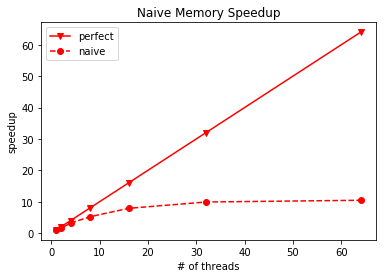
\includegraphics[width=8cm, height=6cm]{naive_memory}
\end{center}

From this chart, we can find that while at first, doubling threads does give solid speedup. However, with an increasing number of threads, the performance improvement it gains when doubling the number of threads decreases really fast. This is due to the fact that the Hermes machine actually contains 4 sockets, and when allocating the memory using naive implementation, all the memory is allocated on one socket. This causes a hotspot and the intense memory accesses to that particular socket from remote cores greatly dragged the overall performance in this halo problem. The solution to solve this problem is by using NUMA library to control the memory allocation, so that it can reduce this problem and provide a better result in performance. 

\section{Optimization}

\subsection{Numa Memory Allocation}

		For the optimized version, we still assigns all the row pointer together. However, different from the original version, the program actually allocates the whole memory onto different nodes evenly using $num\_alloc\_onnode$. This function works the same as malloc, except that it can specified the node the memory is going to be allocated on. Therefore, the memory can then be evenly distributed. However, since we still allocate all the row pointer together as global variables in $main$ function, the thread function used for original version can still apply. Also when using NUMA Memory Allocation, the program also binds the corresponding thread onto the node, on which the rows it needs to compute are allocated. 
		
		More specifically the whole process works as below:
		\begin{itemize}
			\item Divide the rows evenly into num\_of\_threads groups by storing an array containing all the rows that separate two groups.
 
			\item Allocate all the row pointer of two cells in the main memory.
		
			\item Unlike the unoptimized version, allocate each group mentioned above separately onto different numa\_node(group i is allocated on node i \% 8 ) since there are 8 numa\_nodes in total on Hermes
			
			\item Launch thread function

			\item Inside thread function, run $numa\_run\_onnode$ to bind the corresponding thread onto the specific node where its memory is allocated.
			
			\item Join all threads and print the output
		\end{itemize}
		
		 The detailed implementation $**allocate\_cells\_numa$ and $*thread\_compute$ can be found in Appendix $halo.c$. 

\subsection{Runtime data collection}
	Followed are all the timings recorded during testing on Hermes based on different number of threads using optimized memory allocation, with all other settings identical to the timing with unoptimized memory allocation.
	
\begin{table}[ht]
\caption {Optimized Memory Allocation}
\centering
\begin{tabular}{c c c c c c c c}
\hline\hline
num of threads & 1 & 2 & 4 & 8 & 16 & 32 & 64 \\
\hline
 & 1652 & 944 & 520 & 348 & 205 & 143 & 114 \\
 & 1651 & 933 & 522 & 355 & 209 & 147 & 111 \\
 & 1644 & 935 & 529 & 353 & 211 & 148 & 111 \\
 & 1665 & 937 & 522 & 353 & 211 & 142 & 107 \\
 & 1655 & 935 & 533 & 350 & 212 & 139 & 113 \\
\hline
average & 1654 & 936 & 527 & 352 & 210 & 146 & 111\\
\end{tabular}
\centering
\end{table}

\subsection{Analysis}

The following charts are the speedup we get for both versions with different number of threads, given the average runtime of 1 thread as baseline.

\begin{table}[ht]
\caption {Naive Memory Allocation Speedup}
\centering
\begin{tabular}{c c c c c c c c}
\hline\hline
num of threads & 1 & 2 & 4 & 8 & 16 & 32 & 64 \\
\hline
naive speedup & 1.0 & 1.57 & 3.18 & 5.20 & 7.88 & 9.89 & 10.45\\
optimized speedup & 1.45 & 2.57 & 4.54 & 6.87 & 11.45 & 16.47 & 21.09 \\ 
\end{tabular}
\centering
\end{table}

\begin{center}
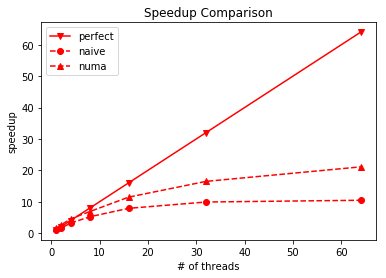
\includegraphics[width=8cm, height=6cm]{speedup}
\end{center}

From these two charts, we can find that while the optimized version still performs much worse than the ideal speedup, it actually has a better performance than the unoptimized version. However, we can still see a significant decrease in performance gain using increasing number of threads. The reason is that, while we do manage to reduce number of remote memory accesses, the intense memory accesses has not changed. With an increasing number of nodes, the parallelism will greatly decrease because of the memory accesses, as the parallel program will need to access memory at the same time, but the memory can only be accessed one at a time, thus hurting the performance.

\section{conclusion}
In this assignment, I have gain solid experience in designing and implementing parallel program using Pthread and NUMA library. The parallel program I implemented shows a substantial performance speedup than the original sequential program with a speedup rate over $20$ times. The optimized version using NUMA is actually twice as fast as the unoptimized version. Also the observation made within two versions indicates the influence of memory hotspot created by parallel accesses is significant in large number of threads on a shared memory machine. While using NUMA can solve part of the problem, the overall speedup is still far from perfect.  
\section{Pledge}

\pledge
\newpage
\section{Appendix}
\subsection{halo.c}
\lstinputlisting[language=C]{halo.c}
\subsection{halo.sh}
\lstinputlisting[language=bash]{halo.sh}

\end{document}
